\chapter{Introduction}
	
	Ce cours est une introduction aux concepts et aux outils mathématiques de base de l'analyse des signaux et des systèmes linéaires. Nous préciserons aussi les conditions d'utilisation de ces outils. Même si ils sont centraux dans le traitement du signal, ils sont indispensables dans d'autres disciplines comme l'électronique, l'automatique, la mécanique, les télécommunications ... En effet, les concepts de systèmes et de signaux sont suffisamment généraux pour s'adapter à des domaines différents. La puissance des notions et des outils que nous présenterons dans ce cours est qu'ils peuvent s'appliquer à des domaines, des grandeurs et des objets physiques complètement différents. Ils constituent des outils largement répandus et utilisés non seulement en ingénierie, mais aussi en recherche.	Les concepts vus dans ce cours seront donc utilisés dans les autres enseignements de la 2e année IMACS, mais aussi des prochaines années, et certainement durant toute votre carrière !
	
	Dans ce premier chapitre, nous allons définir les notions de signal, de traitement de signal et de système dit linéaire à temps invariant. Nous terminerons par une présentation des objectifs pédagogiques du cours, de son organisation et des outils utilisés.
	
	

	
	\section{Le signal}
	
	Dans ce cours, on entend par signal tout phénomène physique qui transporte une information. Il indique l'évolution temporelle, spatiale, d'une ou plusieurs quantités associées à un phénomène physique. Par exemple, il peut s'agir du signal électrique transmis sur un câble réseau ou une onde électromagnétique associée à un réseau WiFi. Les vibrations mécaniques produits par un véhicule, une onde radar, la vitesse de rotation d'un moteur, la température d'une pièce mesurée par un capteur ou un flux de bits lus depuis une mémoire constituent aussi des signaux. Le signal est donc une notion générique provenant de sources physiques très différentes. Pour que ces signaux puissent être traitées et analysées, il faut qu'ils soient mesurés. Pour cette raison, ils sont souvent convertis en signaux électriques.
	
	
	
	
	
	\subsection{Classification des signaux}
	
	Selon sa nature, le phénomène physique, dont le signal constitue la
	signature, peut être exprimé par une fonction mathématique évoluant en
	fonction d'une ou plusieurs variables. Les plus courantes sont des
	variables spatio-temporelles. Dans ce cours, nous traiterons
	principalement de signaux temporels, c'est-à-dire que leur évolution ne
	dépend que du temps, que nous notons s(t). Nous pourrions traiter de la même manière des
	signaux dépendant d'une ou plusieurs variables spatiales, auxquelles on
	pourrait aussi ajouter le temps.
	Considérons que le signal dépend du temps. Nativement, il est exprimé
	dans le domaine temporel, c'est-à-dire que nous pouvons décrire son
	évolution par une fonction dépendante du temps. Nous verrons dans ce
	cours qu'il est possible, via des transformations mathématiques,
	l'exprimer dans un domaine dual, facilitant ainsi son étude ou l'étude
	du système qu'il attaque ou dont il est issu.
	
	Bien que le signal constitue une notion générique qui se ramène à une fonction mathématique, il présente plusieurs caractéristiques que nous allons rapidement présenter.
	
	\subsubsection{Signaux réels ou complexes}
	

	Les signaux physiques sont des signaux réels, c'est-à-dire que les valeurs prises par la fonction $s(t) \in \mathbb{R}$. Cependant, rien n'empêche de définir un signal complexe, dont les valeurs appartiennent à l'ensemble des complexes. L'utilisation des nombres complexes permet la résolution efficace de nombreux problèmes associés à des systèmes physiques. 
	
	\subsubsection{Signaux déterministes ou aléatoires}
	Un signal déterministe présente une évolution parfaitement prédictible. En d'autres termes, on dispose d'un modèle, d'une fonction mathématique permettant de prédire à coup sûr la valeur du signal à un instant donné. \emph{A contrario}, un signal aléatoire n'est pas prédictible. On peut disposer d'un modèle mathématique décrivant l'évolution du signal, mais on ne peut pas prédire exactement la valeur prise à un instant donné. Il faut noter que la plupart des signaux sont aléatoires~: il y a toujours une part d'incertitude dans les phénomènes physiques et les modèles que l'on bâtit pour les étudier sont parfois des approximations. En outre, un signal déterministe n'apporte pas d'informations puisqu'on sait le prédire. 
		
	Le signal déterministe est souvent une abstraction mathématique que l'on rencontre rarement. 
	%TODO rajouter la figure
	%La figure ci-dessous présente la mesure d'un signal électrique produit par un oscillateur. Ce dispositif produit un signal électrique oscillant à une fréquence fixe. Il est donc parfaitement régulier et facilement modélisable par un signal déterministe. Cependant, la mesure montre une fluctuation aléatoire autour de ce signal, liée au bruit intrinsèque du système de mesure et aux perturbations électriques externes qui se superposent. Ainsi, le signal que l'on mesure devient un signal aléatoire.   
	%TODO	Figure signal aléatoire
	
	Malgré la nature aléatoire des signaux, nous nous focaliserons uniquement sur des signaux déterministes dans ce cours. Ceux-ci constituent une abstraction mathématique efficace pour étudier les signaux lorsque la nature aléatoire est négligeable. De plus, cela évite l'introduction d'outils statistiques qui compliquerait inutilement ce cours. Les signaux aléatoires seront abordés en 3e année IMACS.


	\subsubsection{Temps continu ou discret}
	Les signaux physiques présentent une évolution continue en fonction du temps ou de l'espace. Avec l'avènement des systèmes de traitement numérique, l'acquisition de ces signaux requiert de ne prélever qu'un nombre fini d'"échantillons" de ce signal. Un échantillon correspond à une valeur prise par le signal à un instant donné. On parle d'échantillonnage. En d'autres termes, le temps est discrétisé. Cet échantillonnage est généralement effectué régulièrement, selon une période dite d'échantillonnage.
	On parle alors de signaux à temps discret. En effet, un système de traitement numérique met un temps fini pour effectuer une opération. Pendant ce temps, le signal doit rester fixe, d'où la nécessité de ne traiter qu'un échantillon. De plus, le traitement numérique passe très souvent par la mémorisation. Or, une mémoire numérique présente un nombre fini de "cases mémoires". La différence entre signaux à temps continus et à temps discrets est illustrée dans la figure \ref{Fig:Signal_tps_continu_discret}.
	
	\begin{figure}[h!]
          \centering
          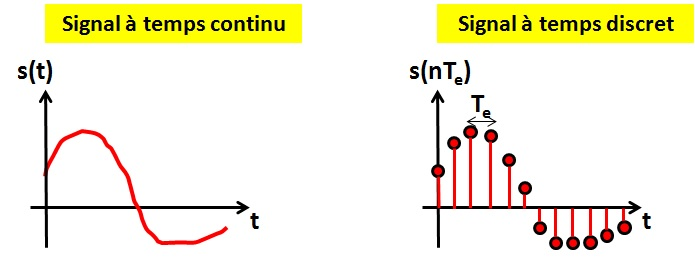
\includegraphics[scale=0.5]{images/Signal_tps_continu_discret.jpg} 
		\caption{Signal à temps continu et à temps discret}	
		\label{Fig:Signal_tps_continu_discret}
	\end{figure}
	
    
	Dans ce cours, nous ne traiterons que des signaux à temps continu. L'effet de l'échantillonnage sur les signaux sera abordé en 3e année IMACS.

	\subsubsection{Signaux à valeurs continues ou discrètes}
	
	La plupart des signaux physiques peuvent prendre une infinité de valeurs à l'intérieur d'un certaine intervalle. On parle alors de signaux à valeurs continues. Cependant, dès qu'un signal doit être traité par un système numérique, celui-ci doit d'abord être encodé sur un nombre fini de bits. Il en résulte un nombre fini d'états que peut prendre le signal. On parle de signal à valeurs discrètes.
	
	En électronique, on distingue ainsi les signaux analogiques, à valeurs et à temps continues, des signaux numériques, à valeurs et à temps discrets.
	
	\subsubsection{Signaux mono-dimensionnels ou multidimensionnels}
	Un signal peut apporter une information sur l'évolution d'une variable ou de plusieurs variables. Par exemple, le signal peut être l'évolution de la position dans l'espace d'un objet. Le signal contiendra trois variables. De même, un signal peut dépendre d'une ou de plusieurs variables caractérisant son évolution~: le temps, l'espace. Dans ce cours nous ne considérerons que des signaux à une dimension.
	

	
	
	\section{Le traitement du signal}
	
 	Le but du traitement de signal est l'analyse et la transformation des signaux en fonctions mathématiques ou paramètres afin d'en extraire l'information. Elle forme une discipline à part entière, et est largement employée dans d'autres domaines, tels que l'électronique, l'automatique, les télécommunications, la thermodynamique, etc.  Elle est en lien avec les mathématiques mais aussi avec le développement de nouveaux moyens de calcul et de traitements numériques.
	Ses finalités sont nombreuses, on peut citer, entre autres~:
	
	\begin{itemize}
		\item l'analyse, c'est-à-dire l'extraction des composantes essentielles portant l'information utile
		\item la mesure, ou l'estimation de grandeurs caractéristiques
		\item la détection et la reconnaissance de signaux, d'informations enfouis
		\item le filtrage, c'est-à-dire l'élimination des composantes "parasites" d'un signal
		\item la restauration d'un signal, liée au processus de filtrage
		\item la synthèse de signaux
		\item le codage, la compression
	\end{itemize}
	
	
	
	Dans ce cours, nous aborderons les outils mathématiques de base d'analyse des signaux. Il s'agit de transformation permettant d'extraire des informations utiles d'un signal. Nous allons notamment aborder l'analyse fréquentielle du signal via la transformée de \Fourier{}. Celle-ci vise à identifier les différentes composantes dites harmoniques qui constituent un signal. L'analyse directe du signal dans le domaine temporel ne permet pas de séparer facilement l'ensemble de ces composantes. L'analyse fréquentielle du signal est souvent l'opération préalable du filtrage, dont le but est l'élimination de signaux indésirables. Bien que son effet soit visible sur l'évolution temporelle d'un signal, un filtre est dimensionné à partir de l'analyse fréquentielle de ce signal.
	
	C'est ce qu'illustre la figure \ref{Fig:analyse_spectrale_voix}. L'évolution temporelle montre un signal complexe, difficilement analysable. L'utilisation d'une transformation mathématique, telle que la transformée de \Fourier{}, met en évidence la présence de plusieurs composantes spectrales, à des fréquences harmoniques, qui forment le signal.
	
	\begin{figure}[h!]
		\centering
		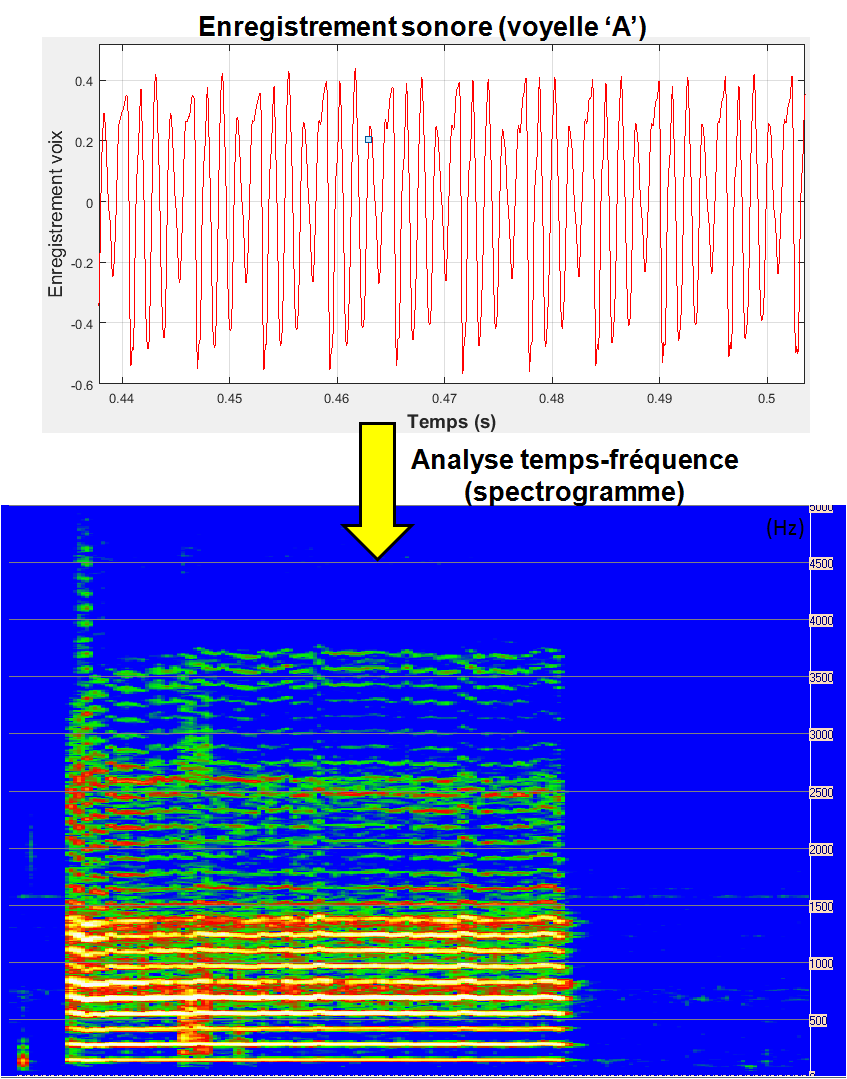
\includegraphics[scale=0.5]{images/spectrogramme_voix.png} 
		\caption{Analyse spectrale de la voix (Logiciel Vocalab, avec la permission d'Etienne Sicard).}	
		\label{Fig:analyse_spectrale_voix}
	\end{figure}
	
	Dans ce cours, la transformée de \Fourier{} ne sera vue que pour des signaux à temps continus. L'impact de l'échantillonnage (ou discrétisation) du signal et sur la transformée de \Fourier{} sera abordé en 3e année IMACS.

	
	\section{Les systèmes linéaires à temps invariant - Réponse d'un système à un signal}
	
	Ce cours a aussi pour but l'étude des systèmes, c'est-à-dire la manière dont ils répondent à un signal d'entrée. Un système est un concept très générique. Ici, nous ne nous intéressons pas à la nature du système et à la compréhension physique de son fonctionnement. Nous pourrons traiter de systèmes électriques, mécaniques, optiques, chimiques, ...	Nous entendons par système le modèle mathématique, abstrait, associé à un objet physique qui décrit son fonctionnement. Il peut être vu comme une "boite" excitée sur son ou ses entrées par un ou plusieurs signaux, comme le montre la \figref{Fig:LTI}. L'évolution de sa ou de ses sorties, que l'on appelle réponse, dépend non seulement du signal d'entrée mais aussi des propriétés du système. Ses signaux d'entrée et de sortie peuvent être représentés par des fonctions mathématiques $x(t)$ et $y(t)$. Du point de vue du traitement du signal, un système transforme les signaux. Son effet peut être modélisé par un opérateur mathématique $L$. Le but de ce cours est de présenter les outils mathématiques permettant de modéliser le système (comment extraire cet opérateur) et de prédire la réponse du système à une excitation donnée. L'objectif est de déterminer un outil mathématique général, fournissant une même méthode de calcul quelle que soit la nature physique du système.
	
	\begin{figure}[h!]
		\centering
		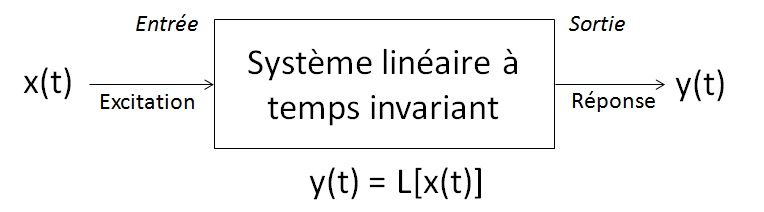
\includegraphics[scale=0.45]{images/LTI.jpg} 
		\caption{Représentation d'un système LTI comme une boîte noire reliant les signaux d'entrée et de sortie par un opérateur linéaire}	
		\label{Fig:LTI}
	\end{figure}


	Dans ce cours, nous traiterons d'une classe de systèmes particuliers, appelés systèmes linéaires à temps invariants (LTI). Les signaux d'entrée $x(t)$ et de sortie $y(t)$ sont reliés entre eux par un ou plusieurs opérateurs linéaires, dont les caractéristiques n'évoluent pas au cours du temps. Si elles sont connues, il devient alors possible de prédire la réponse en sortie du système quelle que soit l'excitation appliquée en entrée. Pour cela, il nous faut déterminer une représentation mathématique de l'effet de ce système, quelle que soit la nature réelle du système. Nous en présenterons deux~: l'effet du système LTI sera modélisé par sa réponse impulsionnelle ou sa fonction de transfert. Les outils mathématiques permettant le calcul de sa réponse seront la transformée de \Laplace{} et le produit de convolution.
	
	Comme pour l'analyse fréquentielle, nous ne considérerons que des systèmes à temps continu. Quasiment tous les systèmes ont une évolution continue dans le temps. Cependant, certains d'entre eux se modélisent efficacement en considérant une échelle de temps discrète. C'est notamment le cas pour les circuits électroniques numériques synchrones, dont le fonctionnement logique est cadencé par une horloge périodique. Les concepts présentés dans ce cours devront être adaptés à cette discrétisation du temps. Ces concepts seront abordés en 3e année IMACS. 
	
	

	
	
	
	\section{Les objectifs pédagogiques}
	L'objectif du cours est le suivant~: présenter les concepts et les outils de base de l'analyse du signal, ainsi que ceux pour le calcul de la réponse des systèmes linéaires à temps invariant.
	
	À l'issue du cours, vous devrez~: 
	\begin{itemize}
		\item (re)connaître les différents types de signaux~;
		\item Calculer le développement en série de \Fourier{} d'un signal périodique et exprimer les coefficients sous ses différentes formes ~;
		\item savoir tracer et interpréter une représentation graphique des coefficients de \Fourier{}~;
		\item calculer la transformée de \Fourier{} (inverse) d'un signal~;
		\item énoncer les principales propriétés de la transformée de \Fourier{} ~;
		\item calculer la puissance, l'énergie d'un signal~;
		\item énoncer les propriétés d'un système linéaire à temps invariant~;
		\item expliquer les notions de réponses naturelles, forcées et d'excitation d'un système naturel, de fréquence naturelle~;
		\item connaître les principales familles d'excitation pour l'analyse des systèmes linéaires (exponentiel complexe, impulsionnelle)~;
		\item calculer la réponse temporelle d'un système linéaire à partir de la transformée de \Laplace{} (inverse)~;
		\item énoncer les principales propriétés de la transformée de \Laplace{}~;
		\item déterminer la réponse harmonique d'un système linéaire à partir de sa fonction de transfert~;
		\item mettre en œuvre le produit de convolution pour calculer la réponse temporelle d'un système~;
		\item déterminer les caractéristiques des filtres linéaires (type, ordre, fréquences de coupure)~;
		\item tracer les caractéristiques d'un filtre dans le diagramme de \Bode{}~;
		\item calculer la corrélation entre deux signaux~;
		\item déterminer la densité spectrale de puissance d'un signal à partir de son auto-corrélation.
	\end{itemize}
	
	
	\section{Organisation du cours}
	Ce cours s'organise de la manière suivante~:
	\begin{itemize}
		\item Nous commençons par l'étude des systèmes linéaires. Le \chapref{chap:lti} est dédié à la définition des propriétés des systèmes LTI, des concepts d'excitation et de réponse. Un préalable au calcul de la réponse d'un système est la recherche de type d'excitations qui facilite cette tache. Nous mettrons en évidence deux types de familles d'excitation~: exponentielle complexe et impulsionnelle. Elles permettront de définir deux manières complémentaires de modéliser un système~: dans le domaine temporel par la réponse impulsionnelle, et dans le domaine fréquentiel par la fonction de transfert.
		\item Le \chapref{chap:laplace} est consacré à la transformée de \Laplace{}. Cet outil, qui transforme une fonction mathématique temporelle en une nouvelle fonction exprimée dans le domaine des fréquences complexes, fournit un moyen très efficace pour calculer la réponse transitoire des systèmes LTI, quelle que soit l'excitation appliquée en entrée.
		\item Le filtrage est abordé dans le \chapref{chap:filtrage}. Les filtres sont des systèmes LTI comme les autres. La spécificité vient de leur utilisation~: l'élimination de composantes fréquentielles indésirables contenues dans un signal. Le dimensionnement d'un filtre passe par une analyse de sa fonction de transfert. Le chapitre présente un outil graphique adapté à l'analyse d'un filtre~: le diagramme de \Bode{}, ainsi que le vocabulaire associé à la caractérisation des filtres.
		\item Le \chapref{chap:series} présente la décomposition d'un signal périodique en une série de termes (co)sinusoïdaux, appelée série de \Fourier{}. Celle-ci forme la base de l'analyse fréquentielle du signal. Après une description des différentes formes prises par la série, les principales propriétés des séries de \Fourier{} sont présentées. Plusieurs exemples de décomposition de signaux en série de \Fourier{} sont donnés. Une représentation du signal en spectre de raies est aussi introduite, fournissant un outil d'analyse graphique puissant.
		\item Les séries de \Fourier{} constituent un formidable outil pour l'analyse des signaux, mais ils sont limités aux signaux périodiques. La transformée de \Fourier{} constitue une extension pour une classe de signaux non-périodiques. Le \chapref{chap:transformee} est dédié à la présentation de la transformée de \Fourier{} et son application. Le chapitre montre aussi que la transformée de \Fourier{} est un cas particulier de la transformée de \Laplace{}.
		\item Le \chapref{chap:temporel} revient sur le calcul de la réponse temporelle des systèmes. Ce point abordé dans le \chapref{chap:laplace} passait par la transformation du signal dans le domaine fréquentiel, via la transformée de \Laplace{}. Dans ce chapitre, on montre comment ce calcul peut être fait directement dans le domaine temporel. Celui-ci nécessite la mise en œuvre du produit de convolution. 
		\item Dans le dernier chapitre, nous revenons sur les concepts de puissance et d'énergie des signaux. Nous présentons les méthodes de calcul dans les domaines temporels et fréquentiels. Nous introduisons un autre outil fondamental pour l'étude de la ressemblance des signaux~: la corrélation. Elle présente aussi un autre intérêt majeur~: sa connaissance permet de déterminer la densité spectrale de puissance d'un signal, donnant la répartition de la puissance du signal dans le domaine fréquentiel.
	\end{itemize}
	
	
	\section{Les outils numériques}
	L'analyse des systèmes et le traitement du signal met en œuvre des calculs potentiellement complexes, ne pouvant pas être toujours résolus à la main voire analytiquement. Des outils numériques sont donc requis.
	Dans les TD et TP associés à ce cours, nous travaillerons avec Matlab\textsuperscript{\textregistered}, outil de référence pour le calcul numérique et le traitement du signal notamment (fr.mathworks.com). Celui-ci est disponible dans toutes les salles d'informatique de l'INSA. Cependant, il fonctionne avec une licence payante. Un équivalent gratuit, quasiment entièrement compatible, est le logiciel Octave (www.gnu.org/software/octave/). Vous pourrez le télécharger et l'installer sur vos machines personnelles.
	